\documentclass{beamer}
\mode<presentation>
\usepackage{amsmath}
\usepackage{amssymb}
\usepackage{adjustbox}
\usepackage{subcaption}
\usepackage{enumitem}
\usepackage{multicol}
\usepackage{mathtools}
\usepackage{listings}
\usepackage{url}
\def\UrlBreaks{\do\/\do-}
\usetheme{Boadilla}
\usecolortheme{lily}

\setbeamertemplate{footline}
{
  \leavevmode%
  \hbox{%
  \begin{beamercolorbox}[wd=\paperwidth,ht=2.25ex,dp=1ex,right]{author in head/foot}%
    \insertframenumber{} / \inserttotalframenumber\hspace*{2ex} 
  \end{beamercolorbox}}%
  \vskip0pt%
}
\setbeamertemplate{navigation symbols}{}

\title{1.7.1 -- Matgeo Assignment}
\author{ai25btech11015 -- M Sai Rithik}
\date{}

\begin{document}
\frame{\titlepage}
\begin{frame}{Question}
Show that the points \((0,0)\), \((2m,-4)\), and \((3,6)\) are collinear, and hence find \(m\), using the rank method.
\end{frame}

\begin{frame}{Step 1: Form vectors}
\[
A = (0,0), \quad B = (2m,-4), \quad C = (3,6)
\]
\[
AB = \begin{bmatrix}2m \\ -4\end{bmatrix}, 
\quad AC = \begin{bmatrix}3 \\ 6\end{bmatrix}
\]
\end{frame}

\begin{frame}{Step 2: Matrix form}
Form the matrix with \(AB\) and \(AC\) as columns:
\[
M = \begin{bmatrix}
2m & 3 \\
-4 & 6
\end{bmatrix}
\]

For collinearity, \(\text{rank}(M) = 1\), i.e. \(\det(M) = 0\).
\end{frame}

\begin{frame}{Step 3: Using RREF}
\[
M=\begin{bmatrix}
2m & 3\\
-4 & 6
\end{bmatrix}.
\]

We use RREF \(M\) and look for when its rank drops below \(2\).

\[
\begin{aligned}
\begin{bmatrix}
2m & 3\\
-4 & 6
\end{bmatrix}
&\xrightarrow{\;R_1 \leftrightarrow R_2\;}
\begin{bmatrix}
-4 & 6\\
2m & 3
\end{bmatrix}
\xrightarrow{\;R_1\gets -\tfrac14 R_1\;}
\begin{bmatrix}
1 & -\tfrac{3}{2}\\
2m & 3
\end{bmatrix}\\[6pt]
&\xrightarrow{\;R_2\gets R_2-2m\,R_1\;}
\begin{bmatrix}
1 & -\tfrac{3}{2}\\
0 & 3(m+1)
\end{bmatrix}.
\end{aligned}
\]

If \(m\neq -1\), the second row has a pivot (divide by \(3(m+1)\)), so the RREF is \(I_2\) and \(\operatorname{rank}(M)=2\).
For the rank to drop (and hence the RREF to have a zero row), we need
\[
3(m+1)=0 \;\;\Rightarrow\;\; m=-1.
\]

When \(m=-1\),
\[
\begin{bmatrix}
1 & -\tfrac{3}{2}\\
0 & 0
\end{bmatrix}
\]
is the reduced row-echelon form (rank \(=1\)).

\end{frame}

\begin{frame}{Conclusion}
\section*{Final Answer}
The given points are collinear when
\[
\boxed{m = -1}
\]

\begin{center}
\end{center}

\begin{figure}[h!]
    \centering
    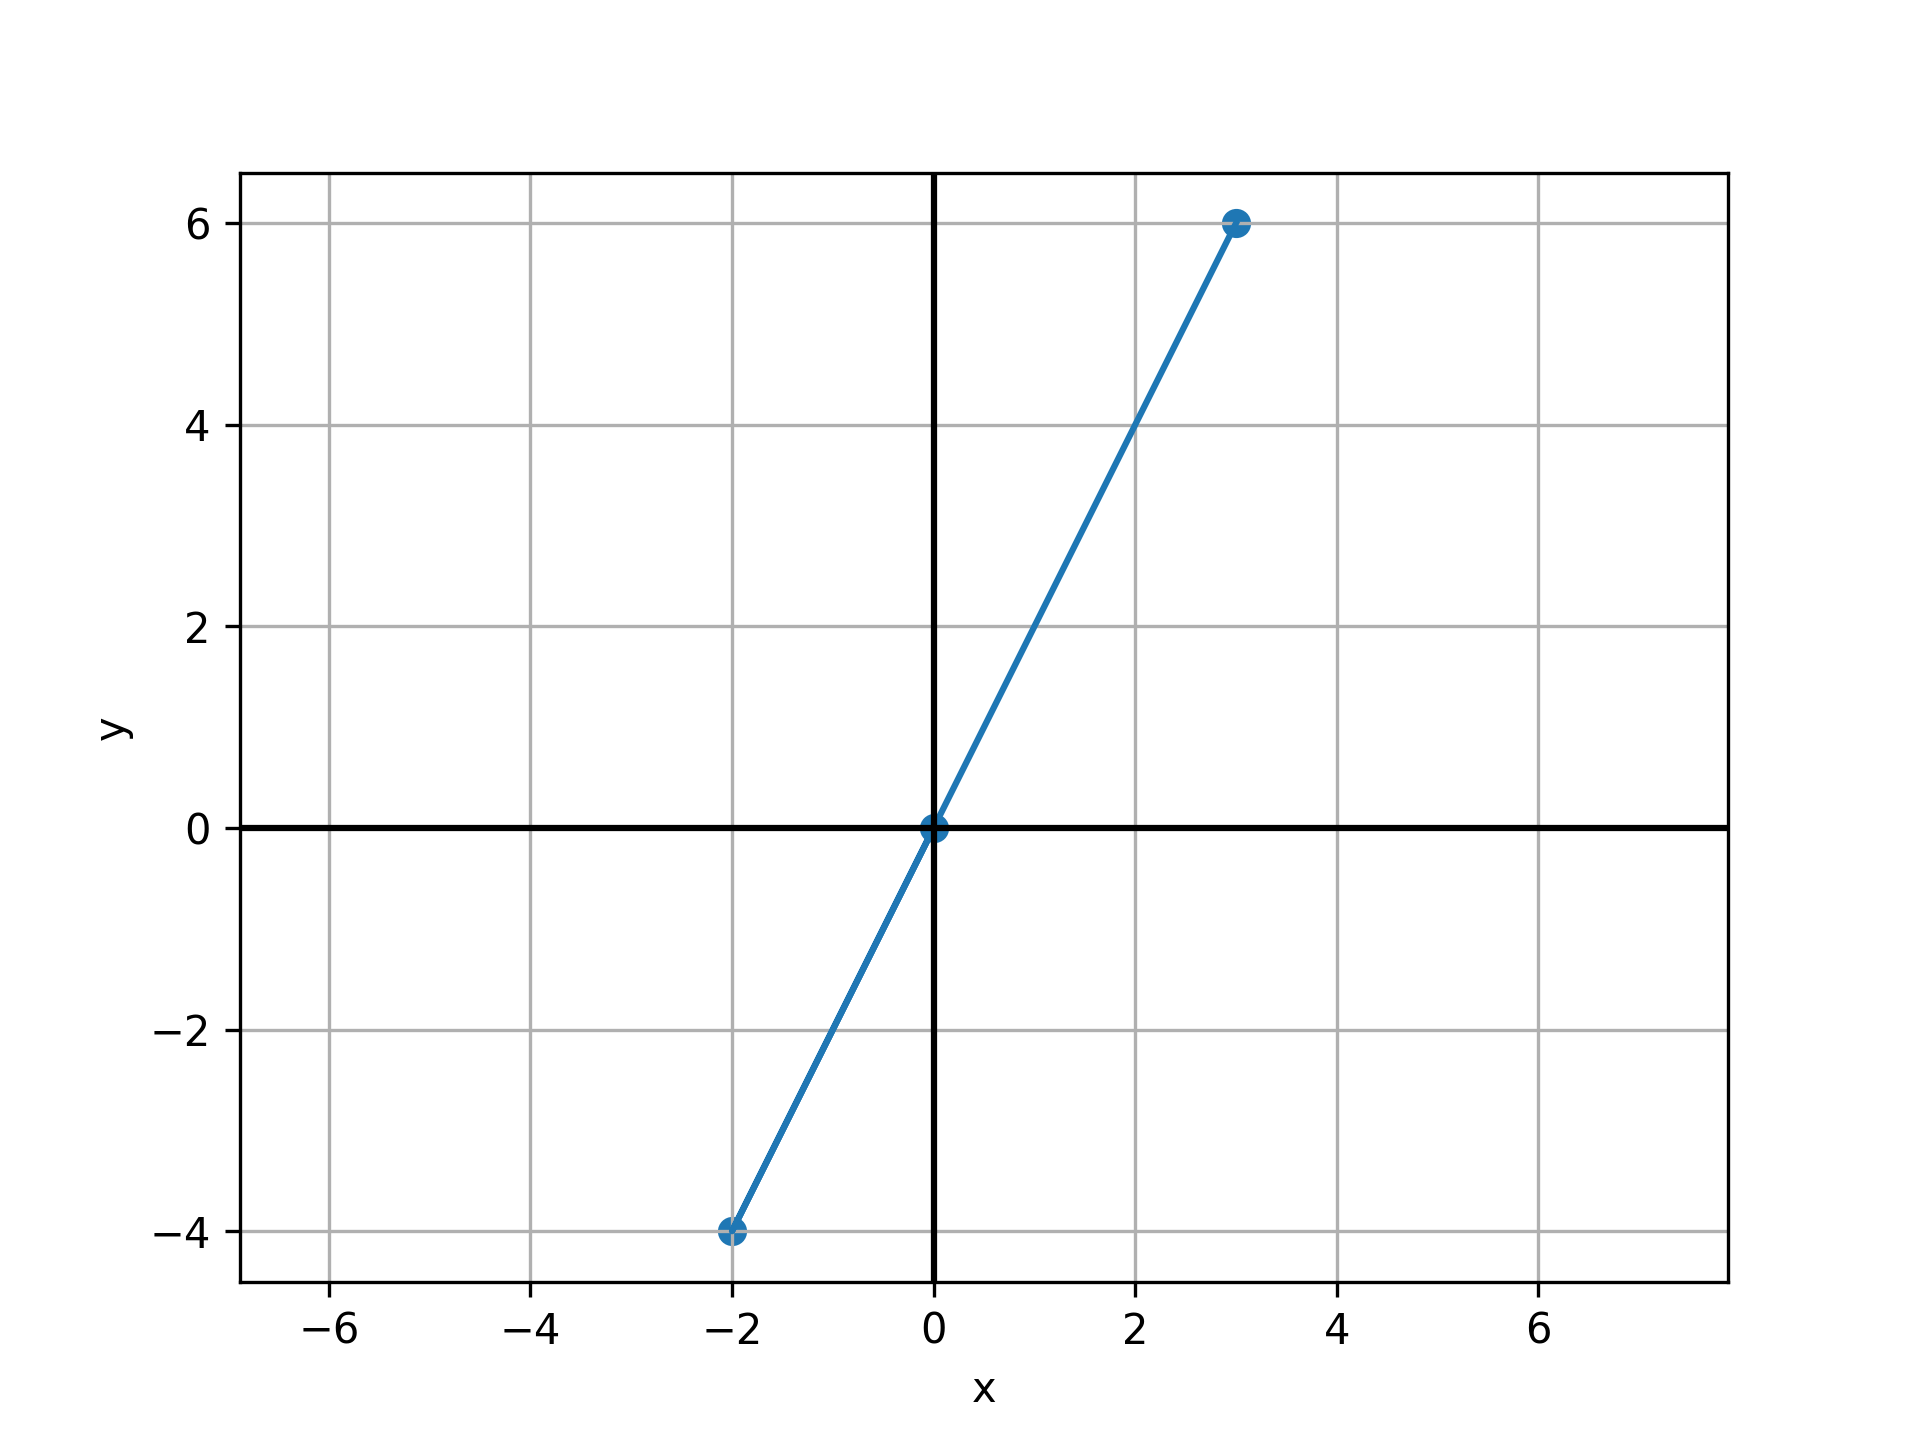
\includegraphics[width=0.65\linewidth]{figs/fig.png}
    \caption{Graph}
\end{figure}
\end{frame}
\end{document}
